\chapter{Konzept} \label{chap:Konzept}
In diesem Kapitel soll das Konzept dieser Ausarbeitung vorgestellt werden. Dieses besteht aus vier Teilen. Zuerst soll das Vorgehen erklärt werden, gefolgt von der Darstellung des Environments und der Agenten. Danach soll im weiteren auf die Datenerhebung eingegangen werden.\\
Ziel dieses Abschnittes ist es, das Vorgehen und alle weiteren dazu benötigten Elemente unabhängig von der Implementierung darzustellen, sodass die Ergebnisse reproduzierbar sind.

\section{Vorgehen} \label{sec:Konzept_Vorgehen}
Das Vorgehen lässt sich am besten mithilfe eines Flussdiagramms darstellen, in welchem die einzelnen Schritte des Vergleichs visuell dargestellt werden.\\
Zu Beginn sei erwähnt, dass die Annahme getroffen wird, dass alle für die Vergleiche benötigten Komponenten, wie z.B. Environment, Agenten und statistische Analysekomponenten, entsprechende der Anforderungen implementiert sind (siehe Abschnitt \ref{chap:Anforderungen}).\\
Als erstes werden die Agenten erstellt (siehe Abbildung \ref{fig:Vorgehen}). Für diese diesen Zweck werden mehrere Klassen mit verschiedenen Hyperparametern generiert bzw. ausgewählt.
Mit dieser Baseline-Agenten-Menge werden nun die weiteren Vergleiche durchgeführt.\\
Zu Beginn werden mithilfe der Evaluationskriterien die zwei optimalen Baseline Agenten bestimmt. Auf diese sollen die Optimierungen angewendet werden. 
Aufgrund der Tatsache, dass das Anwenden der Optimierungen viel Zeit und Ressourcen bindet, sollen diese nur auf die vielversprechendsten Agenten angewendet werden.\\
Der verwendete Algorithmus besitzt dabei keinen Einfluss auf die Auswahl der Agenten, sodass auch zwei DQN oder PPO Agenten optimiert werden können. Genauere Details zur Durchführung der Baseline Vergleiche finden sich im Abschnitt \ref{sec:Konzept_Datenerhebung}.
\begin{figure}[H]
	\centering
	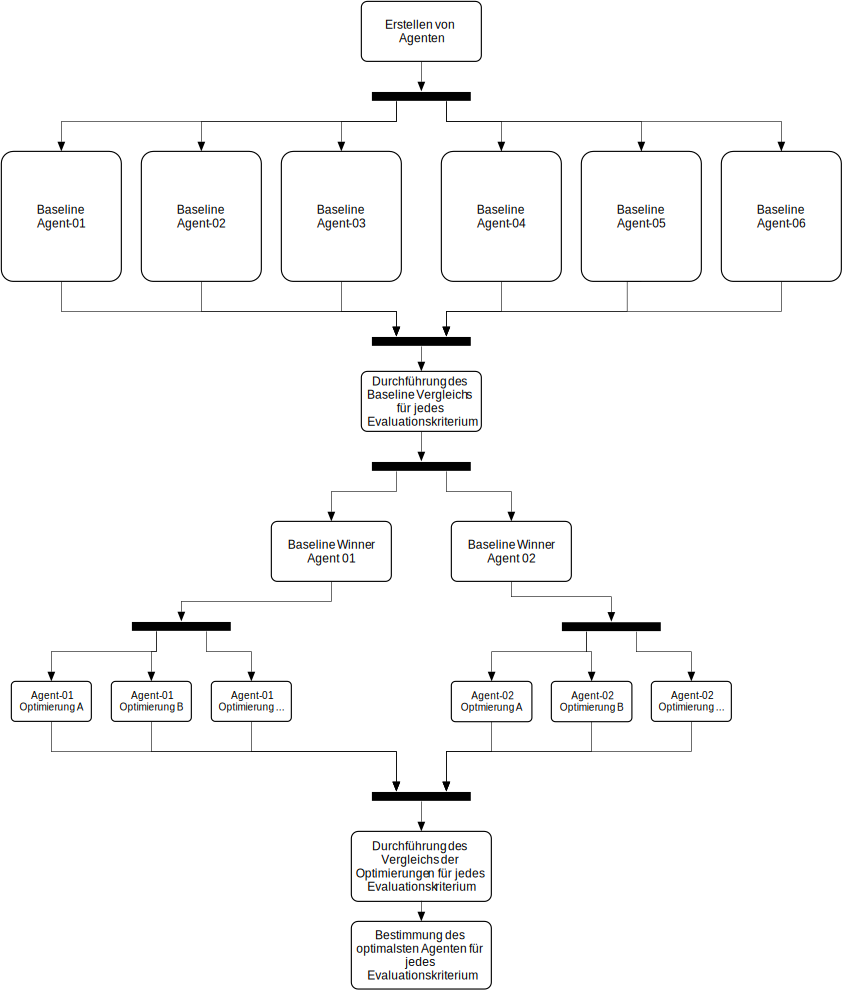
\includegraphics[scale=0.11]{Abbildungen/Vorgehen.png}
	\caption[Flussdiagramm des Vorgehens]{Darstellung des Vorgehens.}
	\label{fig:Vorgehen}
\end{figure}
Basierend auf den beiden Sieger Agenten (Baseline Winner Agent-01 und Baseline Winner Agent-02) der Baseline Vergleiche (siehe Abbildung \ref{fig:Vorgehen}), werden nun die Optimierungen angewendet. 
Mit diesen optimierten Agenten (Agent-01 Optimierung A bis Agent-02 Optimierung B) werden nun die Vergleiche bezüglich jedes einzelnen Evaluationskriteriums (siehe Tabelle \ref{tab:Kriterien}) erneut wiederholt.\\
Im letzten Schritt soll in der gesamt Evaluation der optimale Agent für jedes Evaluationskriterium ermittelt werden. Dabei können dies auch Baseline Agenten sein. Es ist nicht zwingend zugesichert das optimierte Agenten die optimalsten dies.

\section{Environment} \label{sec:Konzept_Environment}
Das Env besteht im wesentlichen aus einer Hauptkomponenten, der Spiellogik, welche von einer Schnittstellen-Komponente umschlossen wird. Diese soll mit einer standardisierten Schnittstelle (siehe \ref{sec:Anforderungen_Schnittstelle}) implementiert werden.\\
Die Spiellogik kapselt die Game-, Player-, Reward-, Observation- und GUI-Komponenten, welche im Folgenden näher erklärt werden.

\subsection{Spiellogik} \label{sec:Konzept_Spiellogik}
\begin{figure}[H]
	\centering
	\def\svgscale{0.17}
	\input{Abbildungen/Spiellogik.pdf_tex}
	\caption[Spiellogik]{Darstellung der Spiellogik mit ihren Unterkomponenten.}
	\label{fig:Spiellogik}
\end{figure}
Die Spiellogik besteht aus den fünf Unterkomponenten, welche im obigen Abschnitt Environment bereits benannt wurden.\\
Die Game-Komponente stellt die Hauptkomponente dar, da sie die eigentliche Aktionsdurchführung implementiert. Sie beinhaltet jeweils Instanzen der Reward-, Obser-vation-, GUI- und Player-Komponenten. Letztere ist eine Datenhaltungskomponente, welche die Daten der Snake, wie z.B. Position oder Ausrichtung (direction) beinhaltet.\\
Die Reward-Komponente bestimmt den auszugebenden Reward nach jeder Aktionsabfertigung. Dieser berechnet sich wie in Abschnitt \ref{sec:Konzept_Reward} angegeben. Zuzüglich wird im Rahmen der Optimierungen A, (siehe Abschnitt \ref{sec:Konzept_Optimierung01}), eine weitere Reward Funktion implementiert.\\
In der Game-Komponente werden wichtige Spielbezogene Daten verwaltet. Zu diesen gehören das Spielfeld (ground), sowie die Form des Spielfeldes (shape) und die Position des Apfels auf dem Spielfeld. Sie beinhaltet viele Methoden, wie z.B. die Aktionsausführung, Observation- und Reward-Erstellung und weitere Routinen.\\
In der Player-Komponente werden Spielerbezogene Daten verwaltet. Zu diesen zählen die Position des Kopfes der Snake, sowie ihrer Schwanzglieder, ihre Ausrichtung (direction), ihre gelaufenen Schritte seit dem letzten Fressen eines Apfels (inter\_apple\_steps), ihr Lebensstatus (is\_terminal), daher ob sie tot oder lebendig ist.\\
Die Observation-Komponente beinhaltet viele einzelne Funktionen zur schrittweisen Erstellung der Observation, wie sie in Abschnitt \ref{sec:Konzept_Observation} erklärt wird.\\
Zur Erzeugung der grafischen Oberfläche implementiert die GUI-Komponente die Funktionalität ein Fenster zu öffnen, welches das Spielgeschehen, daher das Spielfeld (ground), anzeigt und stetig an den neusten Stand anpasst.

\subsubsection{Spielablauf} \label{sec:Konzept_Spielablauf}
\begin{figure}[H]
	\centering
	\def\svgscale{0.11}
	\input{Abbildungen/Spielablauf.pdf_tex}
	\caption[Spielablauf]{Darstellung eines Schrittes in der Spielepisode.}
	\label{fig:Spielablauf}
\end{figure}
Die eigentliche Aktionsabarbeitung wird durch das Aufrufen der step Funktionalität in der Schnittstellen-Komponente (siehe Abschnitt \ref{sec:Konzept_Schnittstelle}) bewirkt. Diese ruft die Routinen zur Erstellung des Rewards (evaluate) und der Observation (observe) auf, welche in der Game-Komponente implementiert sind (siehe Abbildung \ref{fig:Spiellogik}).
Um die Abarbeitung einer Aktion durchzuführen, wird die action Funktionalität aufgerufen. Der Ablauf einer Aktionsabarbeitung ist in der Abbildung \ref{fig:Spielablauf} dargestellt.
Zu Beginn wird überprüft, ob die Snake seit dem letzten Fressen mehr Schritte als die eigentliche Spielfeldgröße gegangen ist. 
Im Rahmen der Bestimmung der Robustheit, wird sich diese im Testverlauf jedoch ändern (siehe Abschnitt \ref{sec:Konzept_Datenerhebung}).\\
Sollte die Snake mehr Schritte gelaufen sein als die Größe des Spielfelds, so wird das Spiel terminiert, da die Snake eventuell in einer Schleife steckt.
Andernfalls wird die Aktion verarbeitet, indem sie die Ausrichtung (direction) der Snake manipuliert wird. Das Spiel Snake besitzt drei Aktionen: turn left, turn right oder do nothing.
\begin{longtable}[h]{|p{4cm}|p{\linewidth - 5cm}|}
	\caption{Kodierung der Aktionen}
	\label{tab:Aktionscodierung} 
	\endfirsthead
	\endhead
	\hline
	Aktion & Erklärung \\
	\hline
	turn left & Die Snake ändert ihre Richtung um 90° nach links. Z.B. Von N $\longrightarrow$ W \\
	\hline
	turn right & Snake ändert ihre Richtung um 90° nach rechts. Z.B. Von N $\longrightarrow$ O \\
	\hline
	do nothing & Die Richtung der Snake wird nicht verändert. \\
	\hline
\end{longtable}
Entsprechend der Tabelle \ref{tab:Aktionscodierung} wird deutlich, dass die Ausrichtung (direction) entweder nur Norden, Osten, Süden oder Westen sein kann.
Als nächstes wird ein Schritt, mit aktualisierten Ausrichtung, hypothetisch durchgeführt. Dabei wird feststellt, ob die Ausführung des Schrittes zum Tod der Snake führt. Sollte dies der Fall sein, so wird der Spielablauf terminiert. Schritte in sich selbst und das Verlassen des Spielfeldes führen zum Tod (siehe Abschnitt \ref{sec:Snake}).\\ 
Anderenfalls wird der Schritt durchgeführt. Dabei wird zwischen zwei Fällen unterschieden.\\
Sollte die Snake einen Apfel gefressen haben, also Kopf und Apfel die selbe Position einnehmen, so wächst die Snake um ein Schwanzglied. Der alte Apfel wird entfernt und ein neuer erscheint, zufallsbasiert, auf einem freien Feld des Spielfelds.\\
Sollte die Snake keinen Apfel gefressen haben, so geht sie einfach den Schritt, es bewegen sich daher alle Schwanzglieder auf die Vorgängerposition, mit Ausnahme des Kopfes, welcher die neue Position einnimmt.\\
Nach der Ausführung einer dieser beiden Fälle, wird die Spieloberfläche und GUI aktualisiert. Nach diesem Schritt ist die Aktionsabarbeitung abgeschlossen.\\
Damit der Agent die momentane Observation und Reward erhält, werden diese in der Reward-Komponente bzw. Observation-Komponente bestimmt und zurückgegeben.

\subsubsection{Reward} \label{sec:Konzept_Reward}
Der Reward wird in der Reward-Komponente, basierend auf dem letzten Zug, gebildet. Dies geschieht nach dem folgenden Vorbild.
Der Standard Reward ist abhängig von drei Faktoren. Dem Fressen eines Apfels, dem Sieg oder Verlust. Sollte keiner dieser genannten Faktoren eintreten, wird ein Reward von -0.01 zurückgegeben. Dies hält den Agenten dazu an den kürzesten Pfad zum Apfel zu finden, da jeder Schritt geringfügig bestraft wird.
War es der Snake möglich einen Apfel zu fressen, so wird ein Reward von +2.5 zurückgegeben, da ein Zwischenziel erreicht wurde.
Sollte die Snake gestorben sein, so wird ein Reward von -10 zurückgegeben, um dieses Verhalten in seiner Häufigkeit zu minimieren.
Hat die Snake alle Äpfel gefressen, sodass das gesamte Spielfeld mit ihr ausgefüllt ist, so wird ein Reward von +10 zurückgegeben, um ein solches Verhalten in seiner Häufigkeit zu maximieren. Dies Snake hat zu diesem Zeitpunkt dann das Spiel gewonnen.\\
Die zweite Reward Funktion wird in Abschnitt \ref{sec:Konzept_Optimierung01} erklärt.

\subsubsection{Observation} \label{sec:Konzept_Observation}
Die Observation, wird in der Observation-Komponente erzeugt und besteht aus der around\_view (AV) un der scalar\_obs (SO). Mithilfe verschiedener Unterfunktionen wird diese generiert.\\
Die AV lässt sich als ein Ausschnitt des Spielfeldes (ground) beschreiben, welcher einen festen Bereich um den Kopf der Snake abdeckt.
Strukturen wie Wände und Teile des eigenen Schwanzes, werden deutlich. Mathematisch ist die AV eine one-hot-encoded Matrix der Form (6x13x13).\\
\\Das One-Hot-Encoding ist ein binäres encoding System. Sollte ein Merkmal vorhanden sein, so wird dieses mit eins codiert anderenfalls mit null. \cite[S. 359 f.]{DRL_Lapan}\\
Dies ist auch der Grund, warum die AV Matrix sechs Channel (zweidimensionale Schichten) besitzt. Diese geben Aufschluss über folgende Informationen:
\begin{longtable}[h]{|p{4cm}|p{\linewidth - 5cm}|}
	\caption{Channel-Erklärung der Around\_View (AV)}
	\label{tab:around_view} 
	\endfirsthead
	\endhead
	\hline
	Channel der Matrix bzw. Erste Dimension (Ax13x13) & Erklärung \\
	\hline
	A = 0 & Die erste Feature Map signalisiert den Raum außerhalb des Spielfelds.\\
	\hline
	A = 1 & Diese Feature Map stellt alle Schwanzglieder mit Ausnahme des Kopfes und es letzten Schwanzgliedes dar. \\
	\hline
	A = 2 & In dieser Feature Map wird der Kopf der Snake dargestellt. \\
	\hline
	A = 3 & Damit gegen Ende des Spiels der Agent noch freie Felder erkennen kann, wird in dieser Feature Map jedes freie und sich im Spielfeld befindliche Feld mit eins codiert. \\
	\hline
	A = 4 & Die vorletzte Feature Map codiert das Schwanzende der Snake. \\
	\hline
	A = 5 & In der letzte Feature Map wird der Apfel abgebildet. \\
	\hline
\end{longtable}
Vorteilhaft an der AV ist, dass, im Gegensatz zu den Obs in den verwandten Arbeiten \cite{Autonomous_Agents_in_Snake_Game_via_DRL} und \cite{UAV}, nicht das gesamte Feld übertragen wird, sondern nur der wichtigste Ausschnitt, was die Menge an zu verarbeiten Daten reduziert.
\begin{figure}[H]
	\centering
	\def\svgscale{0.8}
	\input{Abbildungen/Observation.pdf_tex}
	\caption[Observation]{Partielle Darstellung der verwendeten Observation. Das blaue Rechteck und dessen Schwanz stellt die Snake dar. Schwarzen  wird nicht von der AV abgedeckt, graue liegen innerhalb der AV. Die gelben gestrichelten Linien stellen die Raytracing Distanzbestimmung dar. Der blaue Kreis stellt den Apfel dar und der grüne viertel Kreis oben links symbolisiert den Hunger.}
	\label{fig:Observation}
\end{figure}
Ein Nachteil dieser Obs ist jedoch die Unvollständigkeit. Sollte beispielsweise der blaue Punkt (der Apfel) in Abbildung \ref{fig:Observation} außerhalb des grauen Kasten und daher außerhalb der AV liegen, so bleibt der Agent im Unklaren über den Aufenthaltsort des Apfels.

Aus diesem Grund wurde die AV durch die scalar\_obs (SO) ergänzt.
Die SO beinhaltet skalare Informationen und ist eine Konkatenation aus Raytracing Distanzbestimmung (siehe Abschnitt \ref{sec:Anhang-Implementierung-Distanzen}), Hunger- und Blickrichtungsanzeige (direction). In Quelle \cite{Glassner1989} wird das grundlegende Verfahren, auf welchem die Raytracing Distanzbestimmung basiert, vorgestellt. 
Zuzüglich werden der SO noch zwei Kompasse für relative Positionsinformation zwischen Kopf und Apfel bzw. letztem Schwanzglied hinzugefügt.\\
Letztere sind eindimensionale Vektoren, welche mithilfe des One-Hot-Encoding anzeigen, ob sich das gesucht Objekt relativ zum Kopf oberhalb, unterhalb oder in der selben Zeile befindet (Matrixsicht). Analog verhält es sich mit der vertikalen Sicht.\\
Die Blickfeldanzeige ist ebenfalls one-hot-encoded und stellt mit ihrem Vektor die vier Ausrichtungen Norden, Osten, Süden und Westen dar.\\
Der Hunger ist die Differenz zwischen der Anzahl der gegangenen Schritten seit dem letzten Fressen (inter\_apple\_steps) und der maximalen Schrittanzahl (max\_steps) (siehe Abschnitt \ref{sec:Konzept_Spielablauf}). Zur besseren Verarbeitung für die NNs, wird dieser zudem mit -1 quadriert.
\begin{align}
	\min(2, \frac{1}{inter\_apple\_steps - max\_steps})
\end{align}
Um, mit der Unendlichkeit auftretende, Probleme zu umgehen wird zwei zurückgegeben, wenn die Differenz null wird.\\
In ähnlicher Weise wird mit den Raytracing Distanzbestimmungen verfahren. Bei diesem handelt es sich um acht Distanzmesserlinien, die in 45° Abständen ausgesandt werden, siehe Abbildung \ref{fig:Observation}. Befindet sich das gesucht Objekt in dieser Linie, so wird die Distanz ermittelt und alalog zum Hunger angepasst. Gesuchte Objekte sind Wänden, der eigene Schwanz und der Apfel. Daher wird die Raytracing Distanzbestimmung in einem Vektor der Größe 24 (3 * 8 = 24) gespeichert.

\subsubsection{GUI} \label{sec:Konzept_GUI}
Die graphische Oberfläche oder auch GUI genannt kann optional ein- oder ausgeschaltet werden. Beim Lernen der Agenten bietet es sich beispielsweise an diese auszuschalten, da diese die Lerngeschwindigkeit senkt. Beim Start der GUI wird ein Fenster geöffnet, welches den momentanen Stand der Spielgeschehens anzeigt. Nach jeder Aktionsdurchführung wird die GUI aktualisiert.

\subsection{Schnittstelle} \label{sec:Konzept_Schnittstelle}
Die Schnittstelle umschließt die Spiellogik-Komponente mit ihren Unterkomponenten, um eine standardisierte Schnittstelle zu erzeugen.
\begin{figure}[H]
	\centering
	\def\svgscale{0.15}
	\input{Abbildungen/Wrapper.pdf_tex}
	\caption[Schnittstelle]{Darstellung der Schnittstelle.}
	\label{fig:Schnittstelle}
\end{figure}
Die step Funktionalität (siehe Abbildung\ref{fig:Schnittstelle}) ist für das Aufrufen der Aktionsausführung zuständig. Entsprechend der Anforderung der Standardisierte Schnittstelle (siehe Abschnitt \ref{sec:Anforderungen_Schnittstelle}) gibt sie nur Reward und Observation zurück.\\
Reset setzt den bereits vorhandenen Spielfortschritt zurück (siehe \ref{sec:Anforderung_Reset}).\\
Render ist für die Visualisierung der Spieloberfläche verantwortlich (siehe \ref{sec:visualisierung_Env}).

\section{Agenten} \label{sec:Konzept_Agenten}
In diesem Abschnitt des Konzepts sollen die Agenten inklusive ihrer Netzstruktur vorgestellt werden. Zu diesem Zweck müssen die Algorithmen (DQN und PPO) näher beleuchtet werden.

\subsection{Netzstruktur} \label{sec:Konzept_Netzstruktur}
Zu Beginn soll die Netzstruktur erklärt werden, wobei dies unabhängig von den Algorithmen geschehen kann, da sowohl DQN als auch PPO Agenten das annähernd gleiche Netz nutzen.
Im Rahmen dieser Ausarbeitung soll sich nur auf eine Netzstruktur konzentriert werden, um die Vergleichbarkeit der einzelnen Algorithmen zu erhöhen. Dennoch müssen, aufgrund der Algorithmen, kleinere Anpassungen an den Netzen vorgenommen werden.\\
In den Papers von \cite{Autonomous_Agents_in_Snake_Game_via_DRL} und \cite{UAV} wurden einzig große CNNs (Convolutional Neural Network) genutzt, die viele unnötige Informationen verarbeiten. Zusätzlich können noch Probleme mit variablen Spielfeldgrößen auftreten, sodass in dieser Ausarbeitung auf ein zweiteilige Netzstruktur gesetzt wird. 

\begin{wrapfigure}{r}{5.2cm}
	\centering
	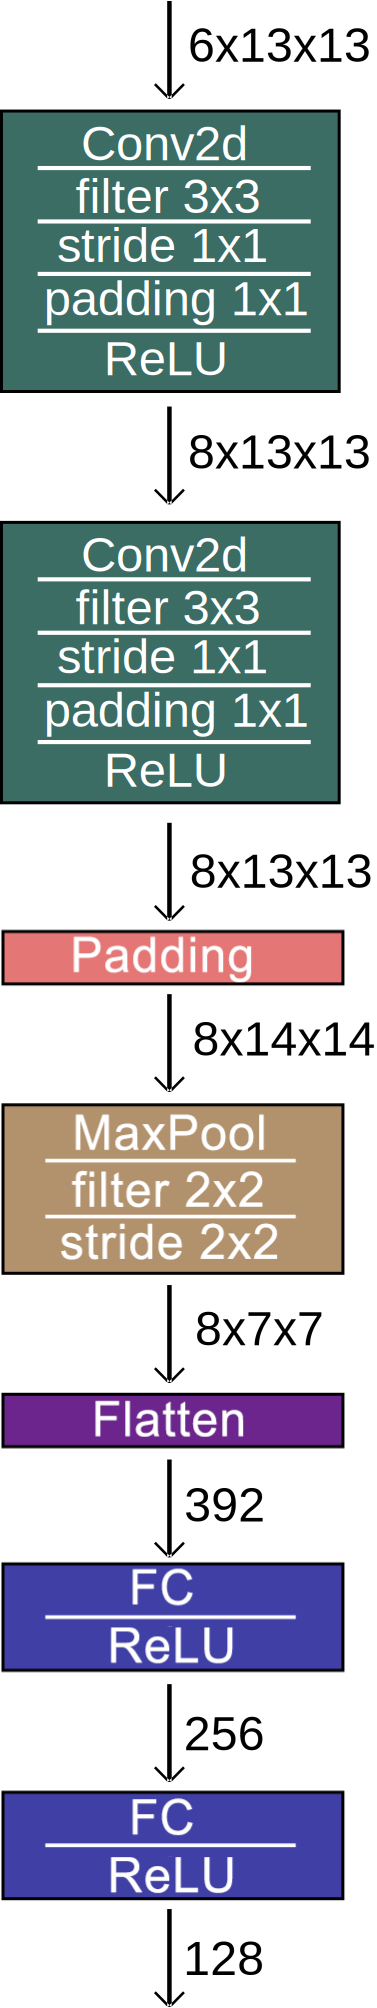
\includegraphics[width=3.0cm, height=15.5cm]{Abbildungen/ConvNet.png}
	\caption[AV-Network]{\\AV-Network}
	\label{fig:AV-Network}
\end{wrapfigure}

Zuerst wird die AV durch das AV-Network geleitet. Diese besteht aus dem AV-Network und Actor-, Critic- oder Q-Tail.
Dabei wird die AV durch zwei Convolutional Layer mit einer ReLU Aktivierungsfunktion propagiert. Dabei erhöht sich die Channel-Anzahl auf acht, wobei eine weitere Erhöhung, aufgrund der bereits sehr stark optimierten AV, nicht nötig ist.\\  
Danach werden allen Feature Maps eine Null-Zeile und Null-Spalte hinzugefügt (Padding), damit beim Max-Pooling, auch die letzten Zeile und Spalte der originalen AV verarbeitet werden. Nach dem max-pooling besitzen die Feature Maps eine Größe 7x7 (Tensor: 8x7x7).\\ 
Dann folgt die Einebnung (Flatten) zu einem eindimensionalen Tensor, welcher daraufhin durch zwei weitere Fully Connected Layer (FC) propagiert wird. Der resultierende Tensor besitzt die Größe 1x128 und ist ein Zwischenergebnis, da dieser nun mit der SO verbunden wird (Join). Der Vorgang ist in der Abbildung \ref{fig:AV-Network} dargestellt.
Da das NN in beide Algorithmen verwendet wird, müssen Netzwerk-Tails für den Actor, Critic und für das Q-Network (Q-Net) definiert werden. Alle unterscheiden sich jedoch nur in ihrer Ausgabe. 
Nachdem der Joined Tensor (1x169), welcher aus dem AV-Networks Output und der SO besteht, durch zwei weitere FC Layer propagiert wurde, benötigt der Actor des PPO Algorithmus eine Wahrscheinlichkeitsverteilung über alle Aktionen. Daher auch die Ausgabe eines Tensors der Größe drei. Um diese Wahrscheinlichkeitsverteilung zu erhalten, wird die SoftMax Funktion angewendet, siehe Abbildung \ref{fig:Critic_Q_Tail} links.\\
Der Critic des PPO Algorithmus verwendet hingegen den Critic-Tail, siehe Abbildung \ref{fig:Critic_Q_Tail} Mitte. Dieser leitet den Joined Tensor durch zwei weiteres FC Layers, wobei das erste eine Aktivierungsfunktion besitzt. Da der Critic für jeden State die Discounted Sum of Rewards bestimmt (siehe Abschnitt \ref{sec:Baseline_Estimate}), gibt dieser einen Tensor mit einem einzigen Wert zurück (Skalar).\\
Der Q-Net-Tail ist in seinem Aufbau sehr ähnlich zum Critic-Tail. Da dieser jedoch die Q-Values für jede Aktion im Zustand bestimmten soll, muss ein Tensor der Größe drei zurückgegeben werden. Von der Struktur der Netze sind Critic- und Q-Net-Tail, mit Ausnahme der Ausgabeschicht, gleich (siehe Abbildung \ref{fig:Critic_Q_Tail} rechts).
\begin{figure}[H]
	\centering
	\includegraphics[width=3cm, height=5.2cm]{Abbildungen/Actor.png}
	\hspace{.1\linewidth}% Abstand zwischen Bilder
	\includegraphics[width=3cm, height=5.2cm]{Abbildungen/Critic.png}
	\hspace{.1\linewidth}% Abstand zwischen Bilder
	\includegraphics[width=3cm, height=5.2cm]{Abbildungen/QNet.png}
	\caption[Critic- und Q-Net-Tail]{Darstellung des Critic-Tail (links) und des Q-Net-Tail (rechts).}
	\label{fig:Critic_Q_Tail}
\end{figure}

\subsection{DQN} \label{sec:Konzept_DQN}
Der DQN Algorithmus und damit auch die Agenten, welche auf diesem basieren, bestehen aus drei Komponenten. Diese ermöglichen die Implementierung der Aktionsbestimmung und Lernprozedur.
\begin{figure}[H]
	\centering
	\def\svgscale{0.18}
	\input{Abbildungen/DQN-Agent.pdf_tex}
	\caption[DQN-Agent]{Darstellung des DQN-Agent mit seinen Komponenten.}
	\label{fig:DQN-Agent}
\end{figure}
Diese Hauptfunktionalitäten sind in der DQN-Komponente eingebettet, welche die zentrale Instanz des DQN darstellt. In ihr werden wichtige Konstanten für den DQN Algorithmus, wie z.B. Gamma, Epsilon (eps), Epsilon-Dekrementierung (eps\_dec), der minimal Wert für Epsilon (eps\_min), die Batch-Size (batch\_size), die maximale Größe des Memory (max\_mem\_size) und die Lernrate (lr), gespeichert.\\
Die Memory-Komponente speichert Erfahrungen des DQN Agenten in einer Ring-Buffer Struktur. Sollte dieser Buffer voll sein, so werden die ältesten Erfahrungen mit den neuen überschrieben. Dies Verfahren wird in Quelle \cite[S. 5]{DBLP:journals/corr/MnihKSGAWR13} dargestellt.
Abzuspeichernde Werte, für jeden Schritt, sind die around\_view (AV), die scalar\_obs (SO) die Aktion (action), der Reward (reward), die Information, ob man sich in einem terminalen Zustand befindet (terminal) und die around\_view (AV\_) und scalar\_obs (SO\_) des Nachfolgezustandes (siehe Abschnitt \ref{alg:DQN}).\\
Die Q-Network-Komponente verwaltet das NN (Q-Network). Dieses wird zur Q-Value Bestimmung und damit zur Aktionsbestimmung genutzt. Es wird durch Lernprozesse aktualisiert.

\subsubsection{Aktionsauswahlprozess} \label{sec:Konzept_Aktionsauswahlprozess_DQN}
Eine genaue Darstellung der Aktionsbestimmung befindet sich in Abbildung \ref{fig:DQN-Aktionsbestimmung}. Um eine Aktion zu bestimmen, muss zuerst ein Zufallswert zwischen null und eins, was den Wahrscheinlichkeiten von 0\% bis 100\% entspricht generiert werden.
\begin{figure}[H]
	\centering
	\def\svgscale{0.13}
	\input{Abbildungen/DQN-Aktionsbestimmung.pdf_tex}
	\caption[DQN-Aktionsbestimmung]{Darstellung der Aktionsbestimmung des DQN-Agent.}
	\label{fig:DQN-Aktionsbestimmung}
\end{figure}
Ist der Zufallswert größer als den momentane Epsilon-Wert, so wird die Aktion durch das Q-Network bestimmt. Anderenfalls wird eine zufällige Aktion ausgewählt. Die Bestimmung der Aktion durch das Q-Network geschieht dabei wie folgt:\\
Die around\_view (AV) und die scalar\_obs (SO) werden durch das Q-Network, entsprechende der Ausführungen in Abschnitt \ref{sec:Konzept_Netzstruktur}, geleitet. Dieses gibt einen Tensor der Größe drei wieder, welcher die Q-Values der Aktionen turn left (0), turn right (1) und do nothing (2) beinhaltet.
Es wird daraufhin die Aktion gewählt, welche dem Index des größten Q-Values entspricht.\\
Sei (0.32, -0.11, 0.45) ein Tensor, welcher vom Q-Network zurückgegeben wurde, dann würde no nothing (2) gewählt werden, da 0.45 der größte Q-Value ist und dieser an Stelle 2 steht.\\
Die oben beschriebene Prozedur stellt den Aktionsauswahlprozess während des Trainings dar. Während Testläufen, wird die Aktion immer durch das Q-Network bestimmt (siehe Abschnitt \ref{sec:Implementierung_act_DQN}).

\subsubsection{Lernprozess} \label{sec:Konzept_Lernprozess_DQN}
Der Lernprozess stellt sich wie folgt dar:\\
Zuerst wird überprüft, ob im Memory genügend Experiences (Exp) gespeichert sind, um einen Mini-Batch mit der zuvor definierten Batch-Size, zu entnehmen. Sollte dies nicht der Fall sein, wird die Methode terminiert. Anderenfalls wird ein Mini-Batch aus zufälligen Exp gebildet. Ab diesem Punkt wird das Verfahren, der Übersichtlichkeit wegen, nur noch für eine einzige Erfahrung beschienen.\\
Danach wird der Q-Value der gespeicherten Aktion $Q(s_i,a_i;\theta_i)$ bestimmt (siehe Gleichung \ref{eq:DQN_Loss}), wobei $s_i$ den State (siehe Abschnitt \ref{sec:State}), $a_i$ die gespeicherte Aktion im Zustand $s_i$ und $\theta$ die Netzwerkparameter des Q-Networks, darstellten. Dieser wird als Q-Eval definiert.\\
Danach werden die Q-Values des Nachfolgezustandes (AV\_ und SO\_) $Q(s',a')$ bestimmt. Sollte der Nachfolgezustand ein terminaler Zustand sein, so werden die Q-Values auf null gesetzt, da diese die zu erwartende Discounted Sum of Rewards angeben (siehe Abschnitt \ref{sec:Return}). In einem terminalen Zustand ist diese Summe gleich null, da keine Zustande mehr besucht werden (siehe Abschnitt \ref{sec:Q-Learning}).\\
Daraufhin wird der maximale Q-Value bestimmt, mit Gamma multipliziert und mit dem erhaltenen Reward addiert $r(s,a) + \gamma \max_{a'}Q(s',a';\theta_{i-1})$ (siehe Gleichung \ref{eq:DQN_Loss}). Dieser Wert wird als Q-Target definiert und soll Q-Eval entsprechen.\\
Am Ende wird der Mean Squared Error zwischen Q-Targets und Q-Evals aus dem Mini-Batch gebildet. Auf Basis dieses Fehlers wird das Q-Network, mittels Backpropagation und Gradientenverfahren, angepasst.

\subsection{PPO} \label{sec:Konzept_PPO}
\begin{figure}[H]
	\centering
	\def\svgscale{0.18}
	\input{Abbildungen/PPO-Agent.pdf_tex}
	\caption[PPO-Agent]{Darstellung des PPO-Agent mit seinen Komponenten.}
	\label{fig:PPO-Agent}
\end{figure}
Der PPO Algorithmus und seine Agenten, bestehen aus vier Komponenten. Diese ermöglichen die Implementierung der Aktionsbestimmung und Lernprozedur.\\
In der PPO-Komponente werden wichtige Konstanten für den PPO Algorithmus, wie z.B. Gamma (gamma), der Epsilon-Clip-Wert (eps\_clip) (siehe \ref{sec:Surrogate_Objectives}), die Anzahl der Trainingsläufe pro Datensatz (K\_Epochs), die Lernrate (lr) und weitere statische Konstanten, gespeichert. Auch werden weitere Unterkomponenten, die im weiteren Verlauf erklärt werden, in dieser Komponente gespeichert.\\
Die Memory-Komponente speichert Erfahrungen eines PPO-Agenten. Abzuspeichernde Werte, für jeden Schritt, sind dabei die around\_view (AV), die scalar\_obs (SO) die Aktion (action), der Reward (reward), die Information, ob man sich in einem terminalen Zustand befindet (terminal) und die logarithmierte Wahrscheinlichkeit der ausgewählten Aktion (log\_prob).\\
Die Actor-Komponente verwaltet das Actor-NN. Dieses wird zur Aktionsauswahl genutzt.
Die Critic-Komponente verwaltet das Critic-NN. Dieses wird einzig von der Lernprozedur verwendet, um die erwartete Discounted Sum of Rewards zu bestimmen. Mit dieser wird im Trainingsverlauf der Value Loss bestimmt (siehe Gleichung \ref{eq:Value_Loss}).

\subsubsection{Aktionsauswahlprozess} \label{sec:Konzept_Aktionsauswahlprozess_PPO}
Der Aktionsauswahlprozess wird in der PPO-Komponente angestoßen. Die AV und SO werden daraufhin durch das Actor-NN propagiert. Der, vom Actor-NN ausgegebene, Tensor der Größe drei (drei mögliche Aktionen), beinhaltet eine Wahrscheinlichkeitsverteilung, auf dessen Basis die nächste Aktion bestimmt wird.\\
Sei (0.05, 0.05, 0.9) die Wahrscheinlichkeitsverteilung über alle Aktionen. Bestimmte man 100 Aktionen unter dieser Verteilung, so würde durchschnittlich 90-mal die Aktion zwei gewählt werden. Aktion null und eins nur rund fünfmal.\\
Wie beim DQN, wird für die Testläufe immer die Aktion ausgewählt, welche die größte Wahrscheinlichkeit vorweist (siehe Abschnitt \ref{sec:Konzept_Aktionsauswahlprozess_DQN}).

\subsubsection{Lernprozess} \label{sec:Konzept_Lernprozess_PPO}
Beim Lernprozess des PPO wird wie folgt verfahren:\\
Zu Beginn werden die Erfahrungen, aus den gespielten Spielen, aus dem Memory (Replay-Buffer) entnommen.
Um den Return zu erhalten, werden die einzelnen Rewards aus dem Memory diskontiert (siehe Abschnitt \ref{sec:Return}).\\
Danach wird die folgende Prozedur mehrmals ausgeführt, um das NN zu trainieren. Danach terminiert die Lernprozedur.
Für ein besseren Verständnis, wird der Ablauf exemplarisch an einer Erfahrung erklärt.\\
Zunächst wird die logarithmierte Wahrscheinlichkeit $\pi_{\theta}(a|s)$ für die gespeicherte Aktion $a$ bestimmt (siehe Abschnitt \ref{sec:Probability_Ratio}). Dazu wird die aus dem Memory entnommene AV (around\_view) und SO (scalar\_obs) durch das Actor- und Critic-NN propagiert. Anschließend wird die logarithmierte Wahrscheinlichkeit der Aktion bestimmt und zusammen mit dem Baseline Estimate (siehe Abschnitt \ref{sec:Baseline_Estimate}) und der Entropie der Wahrscheinlichkeitsverteilungen (siehe Abschnitt \ref{sec:PPO_Training_Objective_Function}) zurückgegeben.
Daraufhin wird die Probability Ratio, aus der soeben bestimmten logarithmierten Wahrscheinlichkeit und der alten logarithmierten Wahrscheinlichkeit des Memory, bestimmt (siehe Abschnitt \ref{sec:Probability_Ratio}).\\
Nachfolgend wird der Advantage, durch Subtraktion des Return mit dem Baseline Estimate, berechnet $\hat{A}(s, a) = R - b(s)$ (siehe Abschnitt \ref{sec:Advantages}).\\
Als nächstes werden die Surrogate Objective Losses Surr1: $r(\theta) \times \hat{A}(s, a)$ und 
Surr2: $\text{clip}(r(\theta), 1 - \epsilon, 1 + \epsilon) \times \hat{A}(s, a)$ bestimmt (siehe Abschnitt \ref{sec:Surrogate_Objectives}), mit welchen der Actor-Loss $L^\text{CLIP} (\theta) = \min(r_{t}(\theta) \times \hat{A}(s, a), \text{clip}(r(\theta), 1 - \epsilon, 1 + \epsilon) \times \hat{A}(s, a))]$ berechnet wird (siehe Gleichung \ref{eq:clip_loss_ppo}).
Um den gesamt Loss des PPO zu bestimmen, wird zusätzlich noch der Value-Loss $L^{\text{VF}} = (V_{\theta}(s)-V^{targ})^2 \text{ wobei } V^{targ} = r(\theta)$ und der Entropy-Loss bestimmt (siehe Abschnitt \ref{sec:PPO_Training_Objective_Function}). Diese werden dann alle zusammengerechnet, entsprechend der Formel: 
$L^\text{PPO} (\theta) = L^\text{CLIP + VF + S} (\theta) = [L^{\text{CLIP}} (\theta) - c_{1}L^{\text{VF}} + c_{2}S[\pi_{\theta}](s)]$ (siehe Abschnitt \ref{sec:PPO_Training_Objective_Function}).\\
Actor- und Critic-NN werden dann mit dem Loss, unter Zuhilfenahme von Backpropagation und Gradientenverfahren, aktualisiert.

\subsection{Vorstellung der zu untersuchenden Agenten} \label{sec:Konzept_Vorstellung_Agenten}
Ein zentraler Aspekt eines Vergleichs von verschiedenen RL-Agenten ist die genaue Definition dieser einzelnen. 
Basierende auf den Grundlagen (siehe Abschnitt \ref{sec:Agent}), sollen hier die zu vergleichenden Agenten vorgestellt werden.\\
Da die ausgewählten Hyperparameter einen immensen Einfluss auf das Verhalten der Agenten besitzen, ist ein Vergleich zwischen DQN und PPO Agenten mit wahllos gewählten Hyperparametern folglich wenig aussagekräftig. Darum sollen im Weiteren die Wahl der Hyperparameter hier begründet werden.\\
\\Wie in der Abbildung \ref{fig:Agenten} zu erkennen ist, können beliebig viele Agenten miteinander vergleichen werden. In dieser Ausarbeitung hingegen sollen 6 Agenten definiert und miteinander verglichen werden.
\begin{figure}[H]
	\centering
	\def\svgscale{0.102}
	\chapter{Agenten}
Ein zentraler Aspekt der eines Vergleiches von verschiedenen RL-Agenten ist die genaue Definition der einzelnen Agenten. Basierende auf den Grundlagen \ref{sec:Agent} soll in diesem Kapitel der Begriff vervollständigt und die zu vergleichenden Agenten sollen vorgestellt werden.\\
Erste statistische Erhebungen haben gezeigt, dass die ausgewählten Hyperparameter einen immensen Einfluss auf das Verhalten der Agenten haben. Bestätigt wird diese Aussage durch die Quelle \cite{Sutton1998}. Ein Vergleich zwischen DQN und PPO mit wahllos gewählten Hyperparametern ist folglich wenig aussagekräftig. Daher ist auch die Definition des Begriffs Agent, welcher nur zwischen DQN und PPO diffenenziert, unzureichend.\\
\\Angebracht wäre eine neuer erweiterte Definition des Begriffs Agent für diese Ausarbeitung. Diese soll um den entscheidenen Faktor der Hyperparameter erweitert werden. Ein Agent wird daher nicht mehr alleinig durch seine Art (Q-Learning oder Policy Gradient bzw. DQN oder PPO) definiert, sondern ebenfalls durch die ausgewählten Hyperparameter.Eine Analogie aus dem Tierreich sollte hier Klarheit verschaffen.\\
\\Im Tierreich gibt es Hunde und Katzen. Diese stellen die RL-Klassen, wie z.B. Q-Learning- oder Policy Gradient Verfahren, dar. Sieht man jedoch genauer hin, so unterscheiden sich die Hunde und Katzen durch ihre jeweiligen Rassen, wie z.B. Pudel und Dalmatiner bei den Hunden und Maine Coons und Norwegische Waldkatzen bei den Katzen. Diese stellen die Algorithmusklassen, wie z.B. DQN oder PPO, dar. Dennoch unterscheiden sich auch Hunde und Katzen der selben Rasse untereinander, nämlich in ihrer DNS. Diese stellt die letzte Differenzierungsebene der Agenten dar. Im Sachzusammenhang stellen die Hyperparameter und Attribute, wie beispielsweise die Netzstruktur, die DNS eines Agenten dar.\\
Soll nun also ein Vergleich zwischen verschiedenen Agenten vollzogen werden, so gilt es als erstes die einzelnen Agenten zu definieren, daher ihre RL-Klasse, Algorithmusklasse und Hyperparameter zu bestimmen.

\section{Agenten}
Im Folgenden werden die einzelnen Agenten, welche untereinander verglichen werden sollen, tabellarisch vorgestellt. Daher wird Aufschluss über Details, wie z.B. die RL-Klasse, Algorithmusklasse, Hyperparameter und die Netzstruktur gegeben.
\begin{longtable}[h]{|p{3.5cm}|p{2.5cm}|p{1.5cm}|p{6cm}|}
	\caption{Agenten}
	\label{tab:Agenten} 
	\endfirsthead
	\endhead
	\hline
	Agentenname & RL-Klasse & Algo-rithmus-klasse & Hyperparameter \\
	\hline
	DQN\_0.99\_64\_5e-6\_2**12\_5e-4 & Q-Learning & DQN & 
	\begin{itemize}
		\item gamma ($\gamma$) =  0.99
		\item batch\_size = 64 = $2^{6}$
		\item epsilon\_decrement = $5\mathrm{e}{-6}$
		\item max\_mem\_size = $2^{12}$
		\item lr = $5\mathrm{e}{-4}$
	\end{itemize} 
	\\
	\hline
	DQN\_0.95\_128\_1e-5\_2**13\_1e-4 & Q-Learning & DQN & 
	\begin{itemize}
		\item gamma ($\gamma$) =  0.95
		\item batch\_size = 128 = $2^{7}$
		\item epsilon\_decrement = $1\mathrm{e}{-5}$
		\item max\_mem\_size = $2^{13}$
		\item lr = $1\mathrm{e}{-4}$
	\end{itemize} 
	\\
	\hline
	PPO\_0.99\_128\_10\_1e-3\_1.5e-3\_0.5\_1e-3\_128\_2**11 & Policy Gradient & PPO & 
	\begin{itemize}
		\item gamma ($\gamma$) =  0.99
		\item K\_epochs = 10
		\item epsilion\_clip = 0.2
		\item lr\_actor = $1\mathrm{e}{-3}$
		\item lr\_critic = $1.5\mathrm{e}{-3}$
		\item critic\_loss\_coefficient = 0.5
		\item entropy\_coefficient = 0.001
		\item batch\_size = 128
		\item max\_mem\_size = $2^{11}$
	\end{itemize} 
	\\
	\hline
	PPO\_0.95\_128\_8\_0.5e-3\_1e-3\_0.5\_1e-4\_64\_2**9 & Policy Gradient & PPO & 
	\begin{itemize}
		\item gamma ($\gamma$) =  0.99
		\item K\_epochs = 10
		\item epsilion\_clip = 0.2
		\item lr\_actor = $1\mathrm{e}{-3}$
		\item lr\_critic = $1.5\mathrm{e}{-3}$
		\item critic\_loss\_coefficient = 0.5
		\item entropy\_coefficient = 0.001
		\item batch\_size = 128
		\item max\_mem\_size = $2^{11}$
	\end{itemize} 
	\\
	\hline
\end{longtable}
	\caption[Agenten]{Darstellung der zu untersuchenden Agenten.}
	\label{fig:Agenten}
\end{figure}
Der erste Agent PPO-01 soll ein langsamer aber stetiger Lerner sein. Mit einer ACTOR Lernrate (ACTOR\_LR) von 2e-4 und einer CRITC-Lernrate von 4e-4 (CRITIC\_LR) wurden Lernraten gewählt, welche, spezifisch für diese Netzstruktur, im Mittelfeld liegen. Ein hoher Wert für GAMMA von 0.99 sorgt für ein zukunftsorientiertes Lernen. Damit der PPO-01 keine zu großen Aktualisierungen der Netze unternimmt, wurde EPS\_CLIP auf 0.15 gesetzt, was, verglichen mit der Literatur \cite[S. 6]{PPO}, recht niedrig ist.\\
\\Der PPO-02 soll ein schnell lernendes Verhalten zeigen. Zu diesem Zweck wurden zwar niedrige Lernraten von 1e-4 (Actor) und 2.5e-4 (Critic) gewählt, jedoch sorgt der relativ große K\_EPOCHS-Wert von zwölf für ein stärkeres Aktualisieren der Netzwerkparameter von Actor und Critic. Dies wird ebenfalls durch den EPS\_CLIP-Wert von 0.25 unterstützt, welcher, nach der PPO Literatur \cite[S. 6]{PPO}, höher als der Durchschnittswert ist. Der GAMMA-Wert von 0.95 bestärkt zudem den schnelleren Lernerfolg, aufgrund der Kurzzeitpräferenz des Agenten.\\
\\PPO-03 soll ein Kompromiss zwischen schnellen Lernen und stetigem Fortschritt sein. Mit mittleren Lernraten von 1.5e-4 (Actor) bzw. 2.5e-4 (Critic) sollte ein schneller und zugleich stetiger Lernfortschritt erzielt werden. Der GAMMA-Wert von 0.95 soll das schnelle Lernen unterstützen. Auch die Werte von K\_EPOCHS mit zehn und EPS\_CLIP von 0.2 werden in der Literatur \cite[Anhang A]{PPO} empfohlen und stellt ein gutes Mittelmaß dar.\\
\\Der DQN-01 ist wieder als langsamer Lerner gedacht. Mit einer großen LR von 8.0e-4 und einem großen GAMMA-Wert von 0.99, wird ein stetiges und zukunftsorientiert Lernen bestärkt. Eine Batch-Size von 128 soll zudem das Lernen beständiger machen. Ein niedriger Werte für EPS\_MIN von 0.001 sollen die Neugierde des Agenten zu Beginn stärken und die Wahl von Zufallsaktionen in späteren Trainingsphasen senken.\\
\\DQN-02 ist wieder als Schnelllerner konzipiert worden. Eine vergleichsweise hohe Lernrate (LR) von 2.0e-4 in Verbindung mit einem kleinen Wert für Gamma von 0.90 soll einen schnellen Lernfortschritt generieren. Dies wird durch eine normale Memory-Size (MAX\_MEM\_SIZE) von 2**11 und die große Epsilon-Dekrementierung (EPS\_DEC) von 5e-5 soll das Lernen weiter beschleunigt und verstärkt werden. Auch sorgt der verhältnismäßig große Wert für EPS\_MIN von 0.0075 für eine schnellerer Exploration und damit für ein schnelles Lernen.\\
\\Der DQN-03 ist wieder als Kompromiss gedacht und besitzt die folgenden Hyperparameter: 
LR = 2.5e-4, GAMMA = 0.95, BATCH\_SIZE = 128, 
MAX\_MEM\_SIZE = 2**11, EPS\_DEC = 4e-5 und EPS\_END = 0.002.

\section{Optimierungen}
In diesem Abschnitt werden die anzuwendenden Optimierungen vorgestellt, welche nach dem Baseline-Vergleich die Leistung in den einzelnen Evaluationskategorien noch weiter verstärken soll. Zu diesem Zweck sollen zwei Optimierungen auf die Baseline Agenten (Agenten ohne Optimierungen) angewendet werden. Die Erstellung von Optimierung A wurde durch die verwandten Arbeiten \cite{UAV} und \cite{Autonomous_Agents_in_Snake_Game_via_DRL} unterstützt. Die Optimierung B wurde nach dem Lesen der Literatur \cite[S. 331 f.]{DRL_Lapan} entwickelt.\\

\subsection{Optimierung A - Joined Reward Function} \label{sec:Konzept_Optimierung01}
Die Joined Reward Function wurde im Paper "`Autonomous Agents in Snake Game via Deep Reinforcement Learning"' \cite{Autonomous_Agents_in_Snake_Game_via_DRL} vorgestellt und im Abschnitt \ref{sec:Paper_1} erklärt. Sie setzt sich aus drei Teilen zusammen. Die Basis bildet ein Distanz Reward, welcher abhängig von der Distanz und Schwanzlänge ist. Um unerwünschte Lerneffekte, von beispielsweise der Neuerzeugung eines Apfels, zu verhindern werden diese Erfahrungen nicht im Memory gespeichert. Zur Verstärkung des Pathfindings wird die Timeout Strategy angewendet, welche den Agenten für nicht zielgerichtetes Verhalten, wie z.B. das unnötige Umherlaufen, bestraft.\\
\\Eine genaue Implementierung dieser vorgestellten Reward Funktion erscheint nicht Sinnvoll, da bereits in der Diskussion (siehe \ref{sec:Paper_1_Diskussion}) zur Quelle \cite{Autonomous_Agents_in_Snake_Game_via_DRL} festgestellt worden ist, dass die Agenten nicht für das effiziente Lösen des Snake-Spiels konzipiert worden sind, sondern für das lange Überleben. Daher muss die Reward Funktion entsprechendes Verhalten begünstigen.\\
Dennoch erscheint die Adaptierung einiger Reward Funktion Elemente als sinnvoll, um eine eigene, für die Performance und Effizienz optimierte, Reward Funktion zu designen.\\
Die Implementierung dieser neuen Reward Funktion findet in der Reward-Komponente statt. 
Dabei wird auf den Distanz Reward der Quelle \cite{Autonomous_Agents_in_Snake_Game_via_DRL} gesetzt, da dieser viele Faktoren des Spiels berücksichtigt, im Gegensatz zur Standard Reward Funktion (siehe Abschnitt \ref{sec:Konzept_Reward}). Dabei wird der Reward wie folgt berechnet:
\begin{align}
	\Delta r(L_t, D_t,D_{t+1}) = \log_{L_t}\frac{L_t + D_t}{L_t + D_{t + 1}}
\end{align}
Wobei $t$ den vorherigen, $t+1$ den aktuellen Zeitpunkt darstellen. $L_t$ ist die Läge der Snake zum vorherigen Zeitpunkt und $D_t$ und $D_{t+1}$ stellen die Distanzen zwischen Snake und Apfel zum vorherigen und aktuellen Zeitpunkt dar.\\
Dieser Distanz Reward wird, wie in Quelle \cite{Autonomous_Agents_in_Snake_Game_via_DRL} dargestellt, auf einen Initial-Wert aufaddiert. Nur setzt sich dieser nicht aus den vergangenen Rewards zusammen, sondern ist in dieser Ausarbeitung fest auf -0.01 gesetzt. Zum Schluss wird dann der Reward noch zwischen -0.02 und -0.005 geclipt, damit der Agent stetig bemüht ist, den optimalen Weg zu finden.
$r_{res} = clip((-0.01 + \Delta r), -0.02, -0.005)$

\subsection{Optimierung B - Anpassung der Lernrate} \label{sec:Konzept_Optimierung02}
Die zweite Optimierung wurde mithilfe von Anregungen aus der Literatur \cite[S. 331 f.]{DRL_Lapan} erzeugt. In dieser wurde die Steigerung der Lernrate diskutiert, um einen schnelleren Lernerfolg zu erzielen. Gegenteilig könnte jedoch die Senkung der Lernrate während des Trainings die Performance und Siegrate verstärken, da die Aktualisierung des NN nicht mehr so stark ausfällt und bestehender Fortschritt damit erhalten bleibt. Darum soll die Lernrate immer dann mit 0.95 multipliziert werden, sobald keine Performance Steigerung in den letzten 100 Epochs bzw. Trainingsspiele erzielt wurde.

\section{Datenerhebung und Verarbeitung} \label{sec:Konzept_Datenerhebung_Verarbeitung}
In diesem Abschnitt soll die Datenerhebung näher thematisiert werden. Daher soll zuerst die Hauptablauf näher erklärt werden, welche Agenten und Env mit einander interagieren lässt. Danach wird die Statistik-Komponente mit ihren Funktionalitäten vorgestellt.

\subsection{Datenerhebung} \label{sec:Konzept_Datenerhebung}
Die Hauptablaufroutine, implementiert den eigentlichen Test und Trainingsablauf.
Um diese auszuführen werden wichtige Hyperparameter des Ablaufs, wie z.B. die zu absolvierenden Trainingsspiele (N\_ITERATIONS), die Spielfeldgröße (BOARD\_SIZE) und weitere Agenten spezifische Hyperparameter, übergeben. Um einen angemessenen Zeitraum für das Lernen zu schaffen, sollen 30.000 Spiele bzw. Epochs für einen Trainingslauf absolviert werden. Die Spielfeldgröße soll dabei standardmäßig, für das Training, bei (8x8) liegen.\\
\\Bei der Datenerhebung ist streng zwischen Test- und Trainingsdaten zu unterscheiden, wobei die Testdaten aus einfachen Spielabläufen bzw. Testabläufen und die Trainingsdaten aus den Trainingsabläufen stammen. Letztere werden wie folgt erhoben.\\
Zu Beginn werden die Datenhaltungsobjekt apples, wins, steps initialisiert, welche für jedes absolvierte Trainingsspiel die, dem Namen des Objektes entsprechenden, Werte speichert. 
Nach der Erstellung des Agenten und Environments startet der Spielverlauf.\\
Dabei wird wie in Abschnitt \ref{sec:Funktionsweise} vorgegangen. Der Agent erhält eine Obs, bestimmt seine Aktion und diese wird sogleich im Env ausgeführt. Danach werden (neue) Obs und Reward sowie weitere Statusinformationen ausgegeben. Diese Daten werden im Memory des jeweiligen Agenten für das sich anschließende Training gespeichert. Dieses wird, wie im DQN-Lernprozess (siehe Abschnitt \ref{sec:Konzept_Lernprozess_DQN}) bzw. PPO-Lernprozess (siehe Abschnitt \ref{sec:Konzept_Lernprozess_PPO}) dargestellt, durchgeführt. 
Danach werden die oben genannten Datenhaltungslisten aktualisiert und die Prozedur beginnt von neuem. Wenn alle Epochs (N\_ITERATION) absolviert wurden, werden die Erhobenen Daten weiter in der Statistik-Komponente verarbeitet (siehe Abschnitt \ref{sec:Konzept_Datenverarbeitung}).\\
\\Die Datenerhebung für Testdaten findet annähernd auf die gleiche Weise statt. Jedoch werden die Daten in nicht aus Trainingsläufen entnommen, sondern aus Testläufen. Bei den Daten handelt es sich um die gleichen, wie in der oben erwähnten Datenerhebung für Trainingsdaten. Der Unterschied zwischen Test- und Trainingsläufen besteht darin, dass die Spielfeldgröße im Rahmen des Testlaufes für die Robustheit variiert wird. Sie kann dabei Größen zwischen (6, 6) bis (10, 10) annehmen. Bei der Messung der Siegrate, Effizienz und der Performance bleibt das Spielfeld jedoch konstant bei einer Größe von (8x8). Anders als bei Trainingsläufen werden zudem bei keine 30.000 Epochs durchgeführt sondern nur 5.000. Dies entspricht ungefähr der Größe einer Datenmenge zur Validierung \cite[S. 134]{DL}.\\
Diese Testdaten werden dann ebenfalls der Statistik-Komponente übergeben (siehe Abschnitt \ref{sec:Konzept_Datenverarbeitung}).
Um die Validität der Statistiken zu garantieren, sollen alle Daten für die Statistiken zwei mal erhoben werden. Damit soll der Anforderung der mehrfachen Datenerhebung entsprochen werden (siehe Abschnitt \ref{sec:Anforderungen_mehrfache_Datenerhebung}). 

\subsection{Datenverarbeitung und Erzeugung von Statistiken} \label{sec:Konzept_Datenverarbeitung}
Nach der Erstellung der Trainings- und Testdaten für jeden Agenten, werden diese, entsprechend der Evaluationskriterien (siehe Tabelle \ref{tab:Kriterien}), verarbeitet. Die Trainingsdaten werden dabei mit Statistiken abgebildet. Die Testdaten werden in Tabellen dargestellt, da diese keinen Verlauf mehr darstellen, sonden nur den momentanen Stand wiedergeben.\\
Diese Verarbeitung der Daten geschieht wie folgt:\\
Die Performance wird anhand der gefressenen Äpfel gemessen. Die Effizienz errechnet sich aus der Anzahl der gefressenen Äpfel (apples) dividiert durch die gegangenen Schritten (steps). Es entsteht daher die Apfel pro Schritt Rate.
Die Robustheit wird gleich der Performance gemessen, nur werden dafür Testdaten, welche auf Spielfeldern mit variabler Größe erhoben worden sind, genutzt. Die Spielfeldgröße soll dabei zwischen (6x6) bis zu (10x10) liegen.
Die Siegrate wird mithilfe der wins bestimmt. Dabei werden die Siege der jeweils 100 letzten Spiele bzw. Epochs gemittelt.\\
Diese Daten werden dann mithilfe von Statistiken ausgewertet. Dabei soll jeweils eine Statistik bzw. Tabelle pro Evaluationskriterium angefertigt werden. Die Daten, welche aus den mehrfachen Erhebungen stammen, sollen, bei der Auswertung, gemittelt werden, um jeweils eine Statistik bzw. Tabelle für jeden Vergleich zu erhalten. Auf diese Verfahrensweise wird jedoch nochmal in der Evaluation (siehe Abschnitt \ref{sec:Evaluation_Datenerhebung}) hingewiesen.
